\documentclass[tikz,border=5pt]{standalone}
\usepackage[T1]{fontenc}
\usepackage{mathptmx}
\usetikzlibrary{arrows.meta,positioning,fit,calc}

\definecolor{roadblue}{RGB}{54,98,132}
\definecolor{roadgreen}{RGB}{82,132,96}
\definecolor{roadamber}{RGB}{176,126,54}
\definecolor{roadgrey}{RGB}{88,94,101}
\definecolor{roadlight}{RGB}{245,247,249}
\definecolor{roadline}{RGB}{72,76,82}

\begin{document}
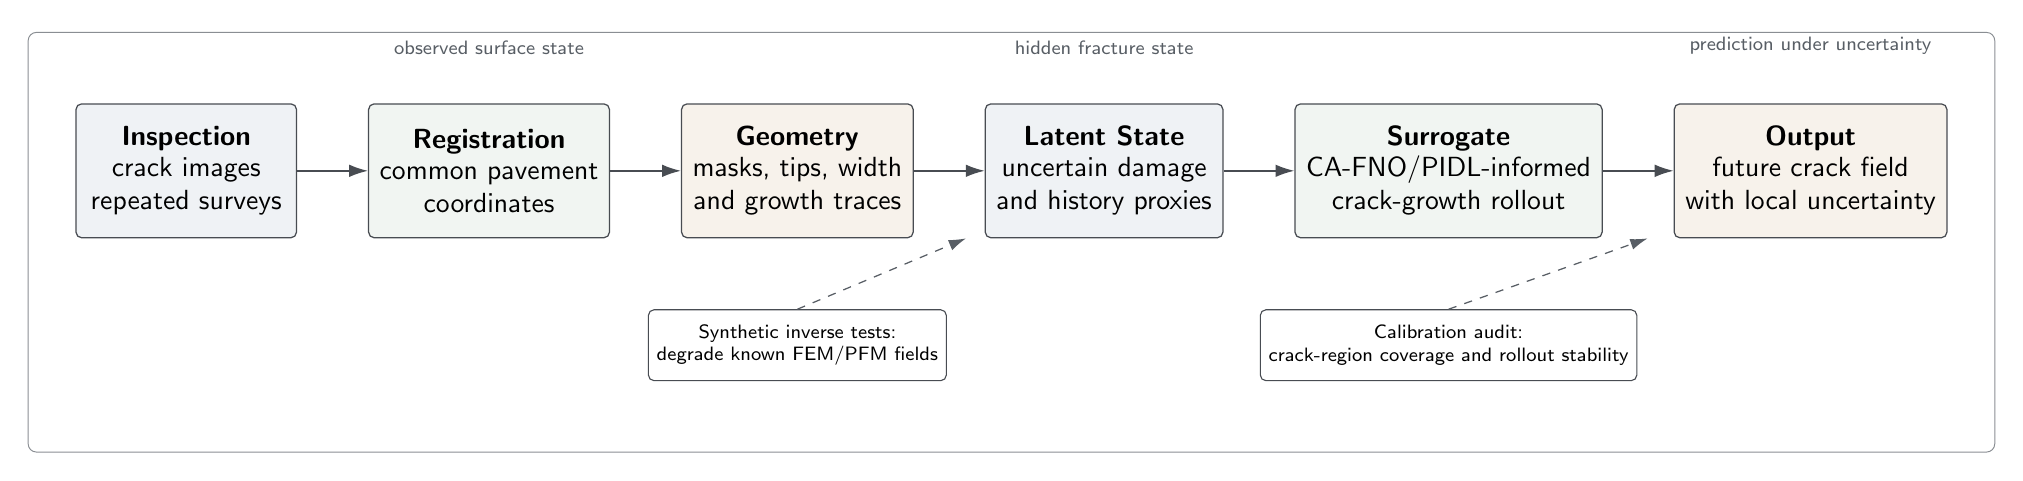
\begin{tikzpicture}[
    font=\sffamily,
    node distance=9mm,
    box/.style={
        rounded corners=2pt,
        draw=roadline,
        line width=0.45pt,
        fill=roadlight,
        minimum width=28mm,
        minimum height=17mm,
        align=center,
        inner sep=4pt
    },
    smallbox/.style={
        rounded corners=2pt,
        draw=roadline,
        line width=0.4pt,
        fill=white,
        minimum width=28mm,
        minimum height=9mm,
        align=center,
        inner sep=3pt,
        font=\sffamily\scriptsize
    },
    arrow/.style={-{Latex[length=2.4mm,width=1.6mm]}, line width=0.55pt, draw=roadline},
    softarrow/.style={-{Latex[length=2.2mm,width=1.4mm]}, line width=0.45pt, draw=roadgrey, dashed},
    phase/.style={font=\sffamily\scriptsize, text=roadgrey, align=center}
]

\node[box, fill=roadblue!8] (inspect) {
    \textbf{Inspection}\\[-1pt]
    crack images\\
    repeated surveys
};

\node[box, fill=roadgreen!8, right=of inspect] (register) {
    \textbf{Registration}\\[-1pt]
    common pavement\\
    coordinates
};

\node[box, fill=roadamber!10, right=of register] (features) {
    \textbf{Geometry}\\[-1pt]
    masks, tips, width\\
    and growth traces
};

\node[box, fill=roadblue!8, right=of features] (state) {
    \textbf{Latent State}\\[-1pt]
    uncertain damage\\
    and history proxies
};

\node[box, fill=roadgreen!8, right=of state] (rollout) {
    \textbf{Surrogate}\\[-1pt]
    CA-FNO/PIDL-informed\\
    crack-growth rollout
};

\node[box, fill=roadamber!10, right=of rollout] (output) {
    \textbf{Output}\\[-1pt]
    future crack field\\
    with local uncertainty
};

\draw[arrow] (inspect) -- (register);
\draw[arrow] (register) -- (features);
\draw[arrow] (features) -- (state);
\draw[arrow] (state) -- (rollout);
\draw[arrow] (rollout) -- (output);

\node[smallbox, below=9mm of features] (synthetic) {
    Synthetic inverse tests:\\
    degrade known FEM/PFM fields
};
\node[smallbox, below=9mm of rollout] (calibration) {
    Calibration audit:\\
    crack-region coverage and rollout stability
};

\draw[softarrow] (synthetic.north) -- ($(features.south)!0.55!(state.south)$);
\draw[softarrow] (calibration.north) -- ($(rollout.south)!0.55!(output.south)$);

\node[phase, above=5mm of register] {observed surface state};
\node[phase, above=5mm of state] {hidden fracture state};
\node[phase, above=5mm of output] {prediction under uncertainty};

\node[
    rounded corners=3pt,
    draw=roadgrey!70,
    line width=0.35pt,
    fit=(inspect)(register)(features)(state)(rollout)(output)(synthetic)(calibration),
    inner xsep=6mm,
    inner ysep=9mm
] (frame) {};

\end{tikzpicture}
\end{document}
